\section{Basic principals}\label{sec:basic_filter}
A digital filter is characterised as an LTI system, previously defined by equation \eqref{eq:LTI_diff_equation_finite}. As described the system is completely characterized by its corresponding impulse response $h[n]$. In terms of the LTI system as a filter the output $y[n]$ is the part of the signal the filters lets through. \\
The output of the system $y[n]$ is defined by the convolution sum of input signal and impulse response of the system: \cite{DTSP, p. 26}
\begin{align}
y[n] = x[n]*h[n] = \sum_{k=-\infty}^{\infty} x[k]h[n-k]
\end{align}    
The frequency response of the system is given by the Fourier transformation of the impulse response, cp. definition \ref{def:Fourier_trans}. Consider the input sequence $x[n]=e^{j\omega n}$ for $-\infty < n <\infty$, then the frequency response is defined as
\begin{align}\label{eq:freq_res}
H(e^{j\omega})=\sum_{k=-\infty}^{\infty}h[k]e^{-j\omega k}
\end{align}
thus the output of the filter becomes 
\begin{align}
y[n]=H(e^{j\omega})e^{-j\omega n} \label{eq:filter_output}
\end{align}
$H(e^{j\omega})$ is in general complex and hence it can be expressed as
\begin{align}
H(e^{j\omega})=|H(e^{j\omega})|e^{j\measuredangle H(e^{j\omega})},
\end{align}  
where $|H(e^{j\omega})|$ and $e^{j\measuredangle H(e^{j\omega})}$ are the \textit{magnitude} and \textit{phase} response of the filter respectively, both real valued and $2\pi$-periodic.\\ 
If the frequency response of a filter is real it is said to have \textit{zero phase}, which is equivalent to the phase response only taking values that are integer multiples of $\pi$, resulting in a straight phase with zero slope. Further if the frequency response can be written in the form 
\begin{align}\label{eq:lin_pha}
H(e^{j\omega})=A(e^{j\omega})e^{j(-\alpha\omega + j\beta)} ,
\end{align}
where $\alpha$ and $\beta$ are constants and $A(e^{j\omega})$ is real, the filter is said to have \textit{general linear phase}. That is because the phase response consists of constant terms added to the linear function making a straight line with slope $\alpha$ except from the discontinuities resulting from jumps of $2\pi$ caused by the 2$\pi$-periodicity. \\
A linear phase response is characterized by a constant \textit{group delay} $\tau(\omega)$:
\begin{align}
\tau(\omega)=-\frac{d}{d\omega}\left\{ \measuredangle H(\text{e}^{j\omega} \right\} = \alpha
\end{align}
The phase response is an expression of how each of the signal components are delayed though the system, where linear phase indicates an equal delay for all components of the signal. To guarantee a constant group delay, $\alpha$, $\beta$ and $h[n]$ has to fulfil the following condition, for all $\omega$ \cite{DTSP, p. 341}.
\begin{align}\label{eq:cons_gro}
\sum_{n=-\infty}^{\infty}h[n]\sin\left(\omega \left(n-\alpha \right) + \beta \right) = 0
\end{align}


\section{Ideal filters} \label{sec:ideal_filt}
When designing filters it is ideal to have constant magnitude and zero phase corresponding to the frequency response. \\ For an ideal selective frequency filter the magnitude response will be constant unity for the frequencies that are wanted to pass the filter referred to as the \textit{bandpass} and zero for all other frequencies referred to as \textit{bandstop}. An example is an ideal lowpass filter with frequency response 
\begin{align}\label{eq:low}
H_{lp}(\text{e}^{j\omega})=
\left\{ \begin{matrix}
1, &\ \left| \omega \right|< \omega_c \\
0, &\ \omega_c < \left| \omega \right| \leq \pi
\end{matrix}\right.,
\end{align}     
where $H_{lp}(\text{e}^{j\omega})$ is $2\pi$ periodic. $\omega_c$ is referred to as the \textit{cutoff frequency}. The lowpass filter selects the frequencies lower than the cutoff frequency and reject the higher frequency components of the input signal. By \eqref{eq:low} it is seen that the lowpass filter is real valued hence has zero phase as expected. \\
The corresponding impulse response are determined by the inverse Fourier transformation on the passband interval.
\begin{align}\label{eq:low_im}
h_{lp}[n]=\frac{1}{2\pi}\int_{-\omega_c}^{\omega_c}\text{e}^{j\omega n} d\omega = \frac{1}{2\pi j n}\left[\text{e}^{j\omega n} \right]_{-\omega_c}^{\omega_c} = \frac{\sin \omega_c n}{\pi n }, \ \  -\infty < n < \infty
\end{align}  \trine{-pi til pi? (peters rettelse) og ret figure!}
By \eqref{eq:low_im} the impulse response is nonzero for $n<0$ hence the filter is noncasual cf. definition \ref{def:causal_system}.\\
Frequency- and impulse response are illustrated on figure \ref{fig:ideal_low}
\begin{figure}[H]
\begin{subfigure}[b]{0.50\textwidth}
        \centering
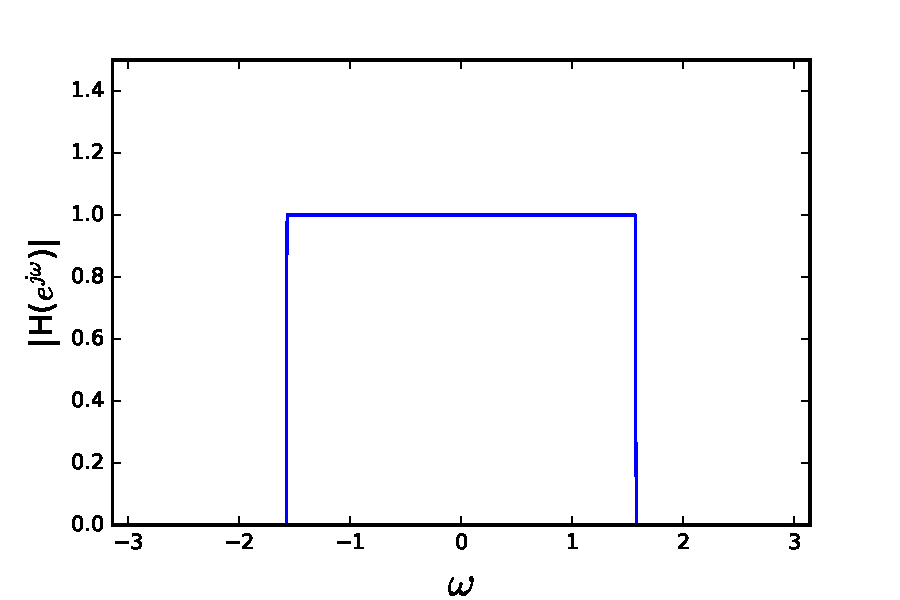
\includegraphics[scale=0.45]{figures/filter_teori/ideal_low2.pdf}
\caption{}
\end{subfigure}
\begin{subfigure}[b]{0.50\textwidth}
        \centering  
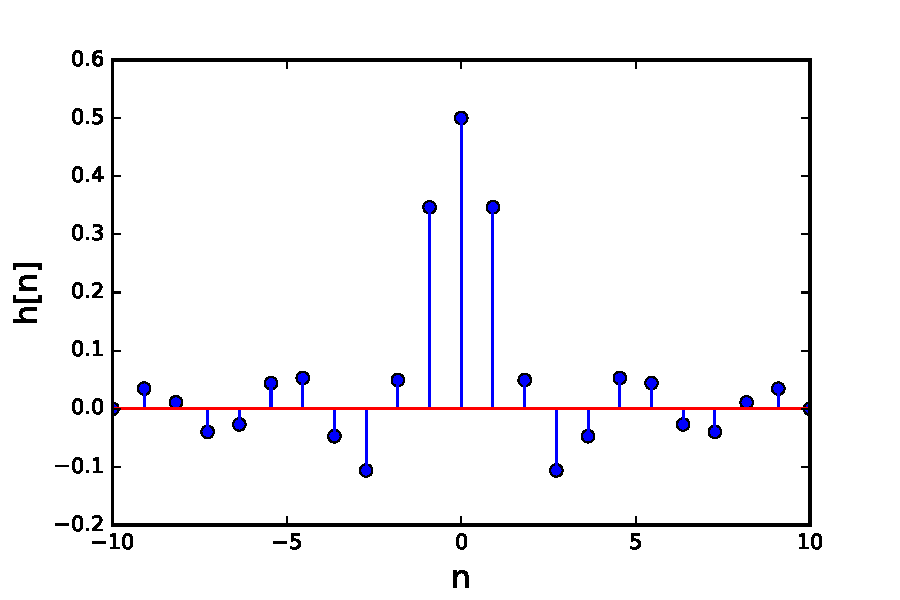
\includegraphics[scale=0.45]{figures/filter_teori/ideal_low1.pdf}
\caption{}
 \end{subfigure}
\caption{ (a) Magnitude response of ideal lowpass filter with $\omega_c = \frac{\pi}{2}$ (b) corresponding impulse response}
\label{fig:ideal_low}
\end{figure}


Analogues of ideal highpass or bandpass filter can be defined, as illustrated on figure \ref{fig:ideal}.\\ 

\begin{figure}[H]
\begin{subfigure}[b]{0.50\textwidth}
        \centering
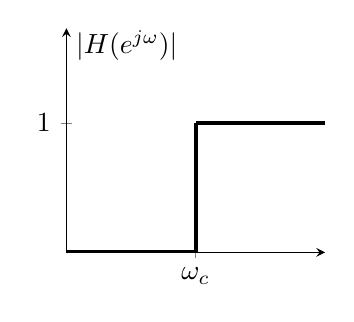
\begin{tikzpicture}[scale=1]
\begin{axis}[
scale=0.5,
unit vector ratio*=1 1 1,
axis lines = middle,
xtick={1.5},
xticklabels={$\omega_c$},
ytick={1.5},
yticklabels={$1$},
xmin=0,
xmax=3,
ymin=0,
ymax=2.6]
\node at (axis cs:0.7,2.4) {$|H(e^{j\omega})|$};
\draw[line width=0.6mm](axis cs:0,0)--(axis cs:1.5,0);
\draw[line width=0.5mm](axis cs:1.5,1.5)--(axis cs:3,1.5);
\draw[line width=0.5mm](axis cs:1.5,1.5)--(axis cs:1.5,0);
\end{axis}
\end{tikzpicture}

\caption{}
    \end{subfigure}
 \begin{subfigure}[b]{0.50\textwidth}
        \centering  
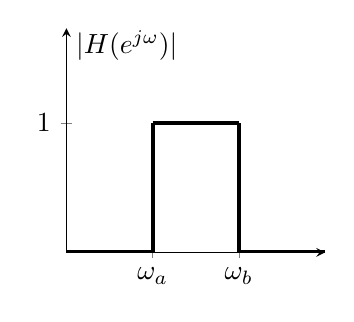
\begin{tikzpicture}[scale=1]
\begin{axis}[
scale=0.5,
unit vector ratio*=1 1 1,
axis lines = middle,
xtick={1,2},
xticklabels={$\omega_a$,$\omega_b$},
ytick={1.5},
yticklabels={$1$},
xmin=0,
xmax=3,
ymin=0,
ymax=2.6]
\node at (axis cs:0.7,2.4) {$|H(e^{j\omega})|$};
\draw[line width=0.5mm](axis cs:1,1.5)--(axis cs:1,0);
\draw[line width=0.5mm](axis cs:1,1.5)--(axis cs:2,1.5);
\draw[line width=0.5mm](axis cs:2,1.5)--(axis cs:2,0);
\draw[line width=0.5mm](axis cs:1,0)--(axis cs:0,0);
\draw[line width=0.5mm](axis cs:2,0)--(axis cs:3,0);
\end{axis}
\end{tikzpicture}
\caption{}
    \end{subfigure}
\caption{Magnitude of ideal (a) highpass filter (B) bandpass filter}
\label{fig:ideal}
\end{figure}
When computing a filter it is not possible to let the output depend on future input, hence noncausal systems are not computable. Zero phase is furthermore not possible for a causal system.
Thus an approximation of an ideal filter can be computed by a casual system with general linear phase.    

\section{FIR and IIR filter} 
Two classes of filter are essential to identify.\\
For all ideal filters discussed in the previous section the impulse response is defined for $-\infty < n < \infty$. Such a filter is specified as an \textit{infinite impulse response (IIR)} filter. In the case of the impulse response being zero outside a finite interval the filter is referred to as a \textit{finit impulse response (FIR)} filter. 
\subsection{Type 1 FIR filter}
As described causal systems with generalized linear phase is wanted. This is possible to guarantee by using specific types of FIR filters.\\
A causal system with generalized linear phase has to fulfil the following relation, cf. section \ref{sec:basic_filter}:
\begin{align}
\sum_{n=0}^{\infty}h[n]\sin\left(\omega \left(n-\alpha \right) + \beta \right) = 0
\end{align}
For a FIR filter to satisfy this relation the following set of conditions has to be fulfilled \cite{DTSP, p.342}:
\begin{align} \label{eq:FIR_con}
&\beta = \left\{ \begin{matrix} 
\pi  \\
0 
\end{matrix}\right. \nonumber  \\ 
&2\alpha = M = \text{an integer} \\ 
&h[n]=h[M-n] \ \text{or} \ h[n]=-h[M-n] \nonumber  
\end{align} 
this implies that $h[n]$ is either symmetric or anti symmetric and that $\alpha = \frac{M}{2}$ becomes the symmetry point. \\
From these conditions four different types of FIR filter with generalized linear phase are defined \cite{DTSP, p. 343}, only the \textit{type 1 FIR filter} will be elaborated here.
A type 1 FIR filter is characterised by having a symmetric impulse response and $M$ being an even integer. By applying the symmetry condition to the definition of the Fourier transformation the frequency response is defined by\trine{rettelse: ref eller lav udledning.}   
\begin{align}\label{eq:type1}
H(\text{e}^{j\omega})=\text{e}^{-j\omega \frac{M}{2}} \sum_{k=0}^{\frac{M}{2}} a[k]\cos \omega k,
\end{align}
where 
\begin{align}
a[k]= \left\{ \begin{matrix}
2h\left[ \frac{M}{2} - k \right], \ \ &\ k=1,2,... , \frac{M}{2}.   \\
h[\frac{M}{2}], \ \ &\ k = 0  
\end{matrix}\right.
\end{align}
By this \eqref{eq:type1} has the form of \eqref{eq:lin_pha} where $A(\text{e}^{j\omega})= \sum_{k=0}^{\frac{M}{2}} a[k]\cos \omega k$ is a real function of $\omega$ and $\beta$ equals either 0 or $\pi$. Hence a constant group delay is achieved.








   
 


 



